
\section*{Exercise 5}
\label{sec:exercise5}

\subsection*{(a)}
\label{sec:a-4}

The dot diagrams\footnote{Jag är lite osäker på hur dot diagram ska se
  ut. Och framföralt hur man gjorde ett i \texttt{matlab}, men jag
  hoppas att detta illusterar det du är ute efter.} are shown in Figure \ref{fig:ex5-marginalplots}. 

\begin{figure}[h]
  \centering
  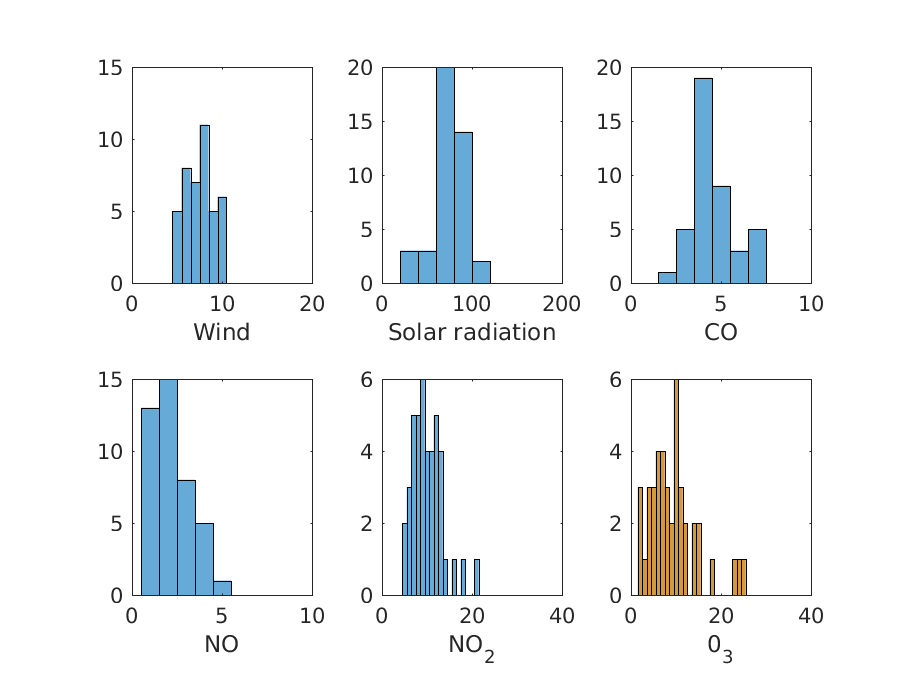
\includegraphics[width=13cm]{ex5-marginalplots}
  \caption{The marginal dot diagrams for all variables}
  \label{fig:ex5-marginalplots}
\end{figure}

\subsection*{(b)}
\label{sec:b-4}

The sample mean is given as
\begin{equation*}
  \bar{x} =
  \begin{pmatrix}
    7.50 & 73.86 & 4.55 & 2.19 & 10.05 & 9.40 & 3.10 
  \end{pmatrix}^T
\end{equation*}
and
\begin{equation*}
  S =
  \begin{pmatrix}
    2.50 & -2.78 & -0.38 & -0.46 & -0.59 & -2.23 & 0.17 \\ 
    -2.78 & 300.52 & 3.91 & -1.39 & 6.76 & 30.79 & 0.62 \\ 
    -0.38 & 3.91 & 1.52 & 0.67 & 2.31 & 2.82 & 0.14 \\ 
    -0.46 & -1.39 & 0.67 & 1.18 & 1.09 & -0.81 & 0.18 \\ 
    -0.59 & 6.76 & 2.31 & 1.09 & 11.36 & 3.13 & 1.04 \\ 
    -2.23 & 30.79 & 2.82 & -0.81 & 3.13 & 30.98 & 0.59 \\ 
    0.17 & 0.62 & 0.14 & 0.18 & 1.04 & 0.59 & 0.48 \\ 
  \end{pmatrix}
\end{equation*}

\subsection*{(c)}
\label{sec:c-4}

The model used was
\begin{equation*}
  y_1 = \beta_0 + \beta_1 x_1 + \beta_2 x_2 + \epsilon,
\end{equation*}
where $\hat{\beta} = (10.1145,\   -0.2113,\    0.0205)$. From here we
can calculate the residual:
\begin{equation*}
  \text{SS}_{\rm E} = 455.1356.
\end{equation*}

Further, we got the following confidence interval with confidence level of 95
\%: $(7.59, 11.71)$. 

\subsection*{(d)}

Here, we propose the linear model
\begin{equation*}
  \begin{pmatrix}
    y_1 \\ y_2
  \end{pmatrix} = 
  BX + E,
\end{equation*}
where 
\begin{equation*}
  X =
  \begin{pmatrix}
    {\bf 1_n} & x_2 & x_2
  \end{pmatrix}.
\end{equation*}
We found that
\begin{equation*}
  B =
  \begin{pmatrix}
    10.11 & -0.21 \\ 
    0.02 & 8.28 \\ 
    -0.79 & 0.10 
  \end{pmatrix}.
\end{equation*}

The confidence region for $x_1 = 10$ and $x_2 = 80$ is shown in Figure
\ref{fig:ex5-ellipse}
\begin{figure}[h]
  \centering
  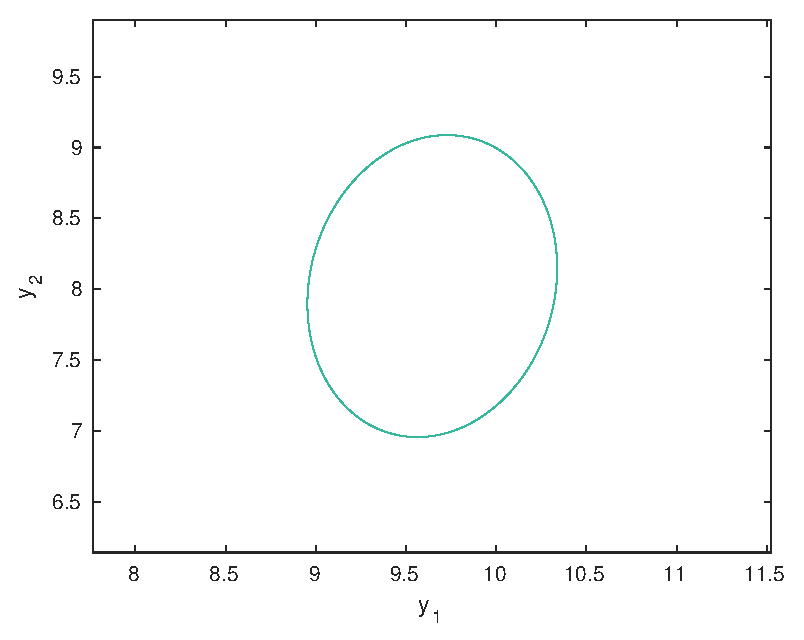
\includegraphics[width=7cm]{ex5-ellipse}
  \caption{The confidence region for $x_1 = 10$ and $x_2 = 80$. }
  \label{fig:ex5-ellipse}
\end{figure}

We can see that the ellipse is covered by 
the confidence interval in Exercise~(c), on the $y_1$ axis.

%%% Local Variables:
%%% mode: latex
%%% TeX-master: "examination"
%%% End:
